\chapter{Game of robber and cops}

We have a given graph $G$. Then 1 robber (\textcolor{Red}{\faCircle}) and $c$ cops (\textcolor{Green}{\faSquare}). This game is for 2 players. Both players take turns. First one plays with cops and the second with robber.

\begin{itemize}[]
	\item \textbf{Start of the game:} First player places cops on vertices of graph $G$. Then second player places the robber in some vertex.
	\item \textbf{Single turn:} First player can with each cop either move to adjacent vertex or stay in the same one. Then the robber can move to adjacent or stay in the same vertex.
	\item \textbf{Goal:} If both cop and robber end up in the same vertex cops have won. Alternatively robber wants to stay as long as possible.
\end{itemize}

\begin{example}
	We have an easy example of the given graph and robber and cops.
	
	\begin{figure}[!ht]\centering
		\begin{tikzpicture}[node distance = 20mm, main/.style = {draw, circle}, thick]
			\node[main] (0) {\textcolor{Green}{\faSquare}};
			\node[main, below of = 0] (1) {\textcolor{Green}{\faSquare}};
			\node[main, left of =1] (2) {};
			\node[main, right of =1] (3) {};
			\node[main, below of =1] (4) {};
			\node[main, left of=4] (5) {\textcolor{Green}{\faSquare} \textcolor{Green}{\faSquare}};
			\node[main, right of=4] (6) {\textcolor{Red}{\faCircle}};
			\node[main, below of =6] (7) {};
			\draw (0) -- (1);
			\draw (1) -- (2);
			\draw (0) -- (2);
			\draw (1) -- (3);
			\draw (0) -- (3);
			\draw (1) -- (4);
			\draw (2) -- (4);
			\draw (3) -- (4);
			\draw (5) -- (4);
			\draw (6) -- (4);
			\draw (7) -- (4);
			\draw (7) -- (6);
			\draw (2) -- (5);
		\end{tikzpicture}
	\end{figure}
\end{example}



\begin{defn}
	The \textbf{cop-number} $\cn(G) :=$ smallest number of cops for which the cops have a winning strategy on $G$. And for class $\mathcal{C}$ of graphs we define $\cn(\mathcal{C}) := \sup \{\cn (G), G \in \mathcal{C}, G \text{ connected}\}$.
\end{defn}

\begin{example}[Cycles]
	For cycles $C_n$ with $n \geq 4$ we can easily see that $\cn(G) = 2$ because we may put two cops in one vertex and then enclose the circle by two pats. Alternatively one is not enough since the robber may only wait and if cop is in the neighboring vertex the robber moves away.
\end{example}

\begin{example}[Int]
	In Int which is class of interval graphs we may find out that $\cn(\text{Int}) = 1$. Firstly we sort the intervals by its left endpoints, then place cop in the leftmost interval. The strategy is either catch a robber or move right to the next interval. If robber could move away the robber must stay way apart to the right or left. But note that if he would be in the left we didn't follow our strategy.
	
	Alternatively we can say the Int has a clique-path decomposition and in each step we are either in the same clique so we can catch the robber or we may move to the next clique.
\end{example}